\section{First Stage Boot Loader (FSBL)}



The FSBL is used to initialize the processing subsystem and prepare it to load a user application or operating system. During the boot process, the BootROM loads the FSBL to the on chip memory. The FSBL can be made to load a bitstream to the programmable logic before loading additional programming to the processing subsystem. \\


\begin{figure}
	\centering
	\begin{tikzpicture}
		\node[state, text width=0.5\textwidth] (bootrom) {BootROM Executes};
		\node[left=1em of bootrom] {Stage 0};
		
		\node[state, text width=0.25\textwidth, below=5em of bootrom.south east, anchor=east] (lockdown) {Lockdown};
		
		\node[state, text width=0.5\textwidth, below=10em of bootrom] (fsbl) {FSBL/User Code};
		\node[left=1em of fsbl] {Stage 1};
		
		\node[state, text width=0.5\textwidth, below=of fsbl] (os) {Operating System};
		\node[left=1em of os] {Stage 2};
	
		\draw[pil] ($ (bootrom.south east) - (0.125\textwidth,0) $) -- ($ (lockdown.north east) - (0.125\textwidth,0) $) node[right, midway] {Failure};
		\draw[pil] ($ (bootrom.south) - (2,0) $) -- ($ (fsbl.north) - (2,0) $) node[right, midway] {Success};
		\draw[pil] ($ (fsbl.south) - (2,0) $) -- ($ (os.north) - (2,0) $);
		\draw[pil] (lockdown) -- ++(0, -1) -- ++(2,0) node[right, near end, xshift=2em] {Error code generated};
	
		\draw[decorate, decoration={brace, raise=0.5em, amplitude=1em}, very thick] (fsbl.north east) -- (os.south east) node[right, anchor=west, midway, xshift=2em, text width=9em] {The FSBL/User/ Application code can clear, program and enable the PL.};
	
	\end{tikzpicture}
	\caption{PS/PL Boot Process for Hardware and Software\citep[p. 151]{zynqtrm:15}}
\end{figure}



% -----------------------------------------------------
% 		Create FSBL Project
% -----------------------------------------------------
\section{Create FSBL Project}

Within an exported hardware SDK workspace, an FSBL project can be automatically generated. The SDK uses the hardware definition files to determine the configuration data for the FSBL. The hardware definition files also contain initialization code that can be used to build make custom builds of U-Boot which, combined with the FSBL, can be used to generated a Snickerdoodle boot image.


%%%-------- FSBL Application Project Platform and BSP ----------
\subsection{FSBL Application Project Platform and BSP}

As shown in \figref{fig:createfsblproj}, the FSBL can be created in the same way as a bare-metal application project by navigating to \menupath{File, New, Application Project}. From the New Project dialog, select a \menupath{standalone} platform. A project name can be entered from this interface.


\begin{figure}
	\centering
	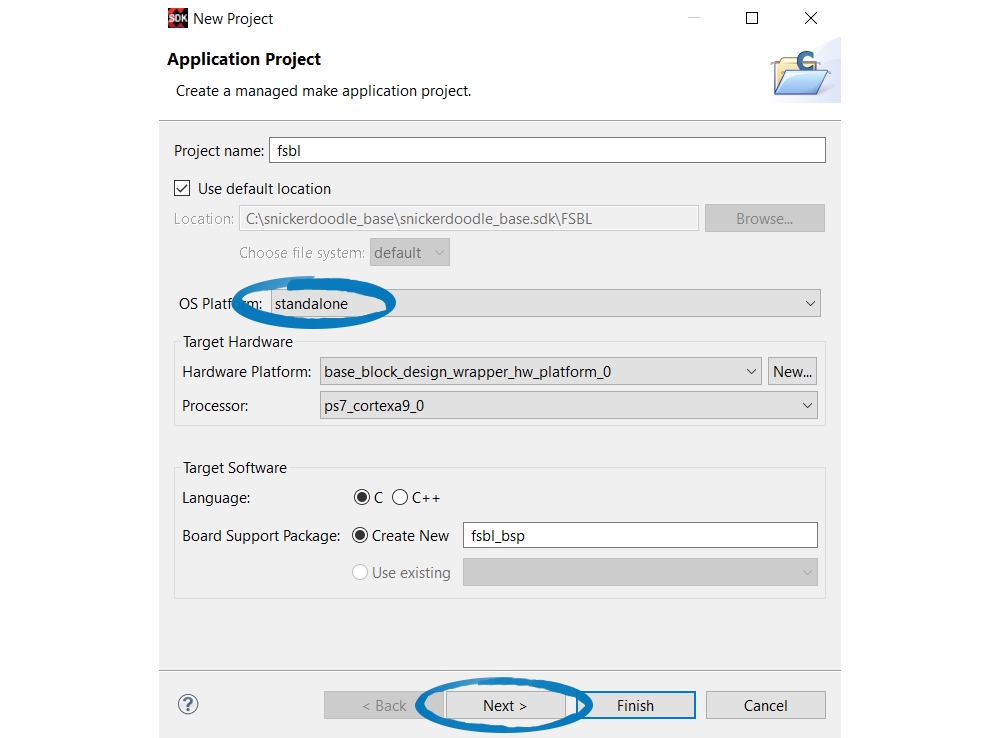
\includegraphics{images/sdk/FSBL_Project.png}
	\caption{Create a New FSBL Project in SDK}
	\label{fig:createfsblproj}
\end{figure}


%%%-------- FSBL Application Project Template --------
\subsection{FSBL Application Project Template}

By clicking \menupath{Next>}, a project template option dialog (\figref{fig:createfsbltemplate}) will appear. Within this dialog window, an FSBL project template can be selected, which will use the hardware configuration to generate the initialization code for the FSBL. Clicking \menupath{Finish} will complete the project generation and build the FSBL code from the workspace hardware configuration.

\clearpage
\begin{figure}
	\centering
	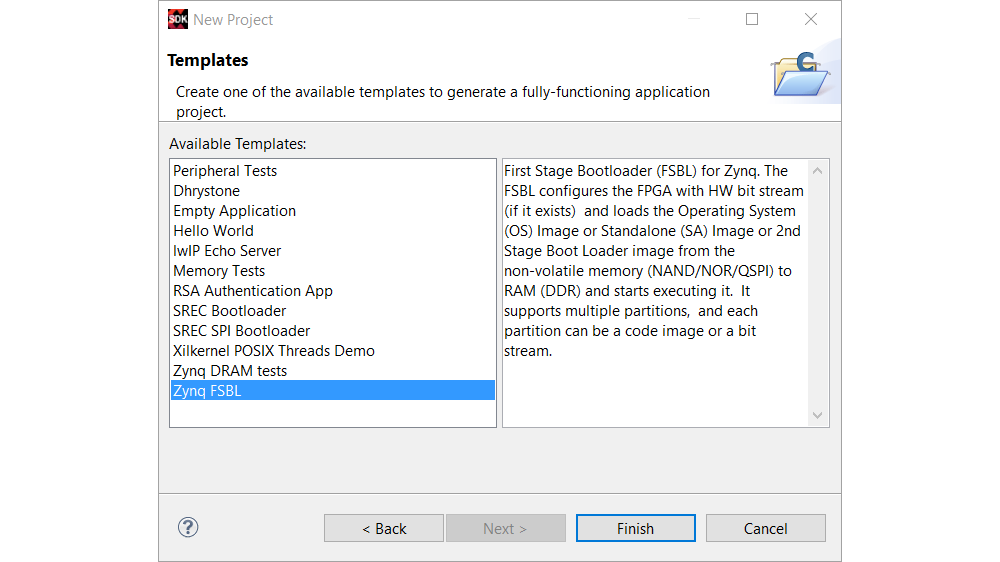
\includegraphics{images/sdk/FSBL_Template.png}
	\caption{Create FSBL Project from Template in SDK}
	\label{fig:createfsbltemplate}
\end{figure} 

The FSBL template will read the hardware definition that was exported by Vivado and generate code required to configure the processing subsystem. A set of initialization files will be generated which is used by the FSBL to configure the processing subsystem before handing off execution to a second stage bootloader or user application. These initialization files can also be used to initialize the processing subsystem for bare-metal applications or custom operating systems.

\begin{figure}
	\centering
	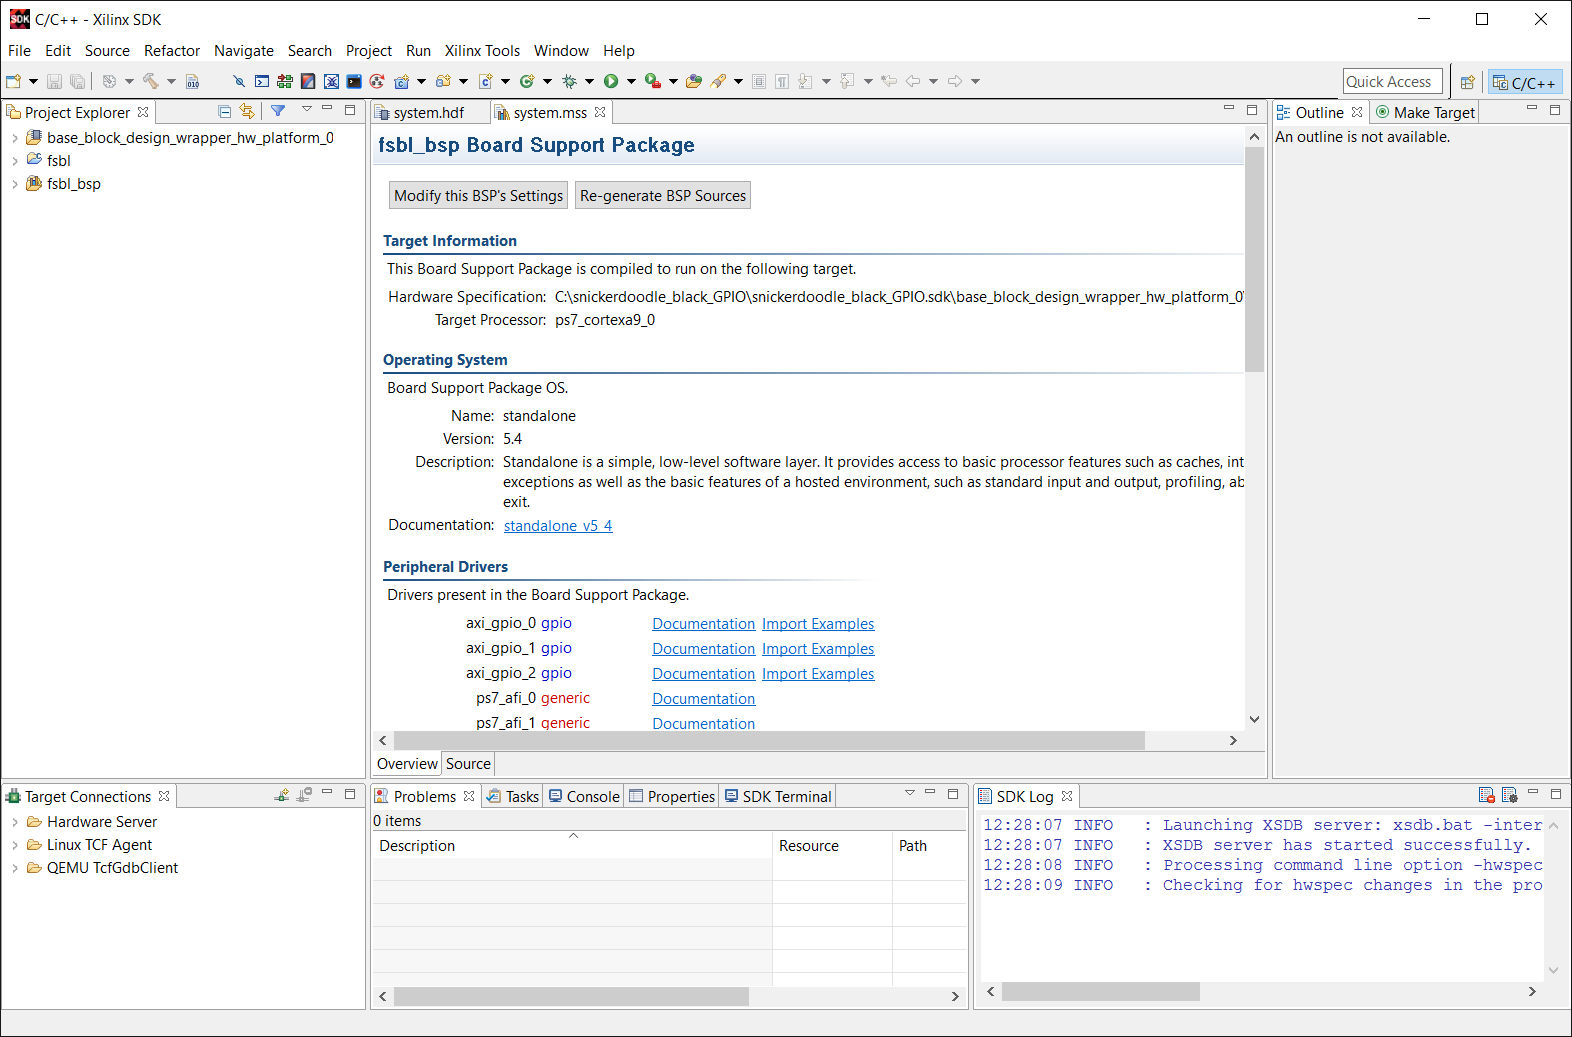
\includegraphics{images/sdk/hardware_exported_workspace.png}
	\caption{Exported Hardware Workspace with FSBL Project and BSP}
	\label{fig:workspacefsbl}
\end{figure}


\section{Boot Image (\file{BOOT.bin})}
\label{ch:inithardwaresys}

Whether using a pre-built hardware configuration or working with a custom solution, a bootable image must be produced which initializes the processing subsystem and (optionally) the programmable logic. The specifics components that are included in a boot image depend heavily on the requirements of the application. While a single boot image configuration cannot be made to suit all applications, a generic boot configuration can be used as a starting point for customization. \\


The boot image should contain, at least, all of the information required to initialize the processing subsystem, typically through a combination of FSBL and U-Boot boot loaders. A bitstream which defines the programmable logic configuration can be loaded upon boot by building the bitstream into the boot image or a minimal boot image can be used if the bitstream is to be loaded from user/application space. 


%-----------------------------------------------------------
% 		Boot Information File
%-----------------------------------------------------------
\section{Boot Information File (\file{.bif})}

The components of a boot image are defined by a boot information file (\file{.bif}). The structure of the \file{.bif} will depend on the specific application details of the system. Typical components for creating a boot image are as follows:

%\margininfonote{Chapter 6 in the \cite{zynqtrm:15} \href{http://www.xilinx.com/support/documentation/user_guides/ug821-zynq-7000-swdev.pdf}{Zynq-7000 All Programmable SoC Software Developers Guide} has more detailed information about the boot process and components of the boot image.}

\begin{description}
	\item[\texttt{FSBL}] - First stage boot loader (FSBL). Responsible for loading the bitstream (if one exists), loading into memory and handing off the boot process to the second stage bootloader. The FSBL should always be specified with the \textit{bootloader} tag in the \file{.bif}.
	\item[\texttt{U-Boot}] - Second stage boot loader. Responsible for loading Linux system components (devicetree, uImage, file system)
	\item[\texttt{Bitstream}] - The bitstream to be built into the boot image.
	\item[\texttt{Device Tree}] - The Linux devicetree to be loaded by FSBL or U-Boot.
	\item[\texttt{Kernel}] - Linux kernel image to be loaded by FSBL or U-Boot.
\end{description}




%%%--------- Small Initialization Boot Image ----------
\subsection{Small Initialization Boot Image}

A very small boot image can be built using FSBL and U-Boot. An image with this configuration can be used to load application or operating system images from a specified boot medium (\ie microSD, QSPI). This boot image provides no application programming, on it's own. An advantage of this approach is modularity and flexibility of the other system components and choice of boot medium. \lstref{lst:smallbootimage} shows the \file{.bif} structure for producing a small boot image.


\begin{lstlisting}[%
	style=text,
	caption=Minimal Boot Image with FSBL and U-Boot,
	label=lst:smallbootimage
]
image : {
        [bootloader]fsbl.elf
        u-boot.elf
}
\end{lstlisting}


%%%---------- Load Image Using FSBL -----------
\subsection{Load Images Using FSBL}

\margininfonote{The uImage.bin file specified in the \file{.bif} is simply a uImage that has been renamed with \file{.bin} for compatibility with \cmdstr{bootgen}}

An entire standalone image can be produced with all of the components required to boot Linux. The first configuration of such a boot image is specified to load the system components into memory using FSBL. With this specification, the Linux components will be loaded into memory before FSBL hands off execution to the second stage boot loader (U-Boot). The \texttt{load=0xXXXX} tag is added to any images that should be loaded by the FSBL during the boot process. This will place the image in the specified memory location, from which the system can be booted using \cmdstr{bootm} from U-Boot. \lstref{lst:biffsblpreload} shows an example \file{.bif} specification with the memory addresses to load the Linux components. With this configuration, the images are pre-loaded and thus the boot process is well-defined and inflexible but simple.


\begin{lstlisting}[%
	style=text,
	caption=Load Linux Components Using FSBL,
	label=lst:biffsblpreload
]
image : {
        [bootloader]fsbl.elf
        u-boot.elf
        [load=0x2a00000]devicetree.dtb
        [load=0x2000000]uramdisk.image.gz
        [load=0x3000000]uImage.bin
}
\end{lstlisting}

%%%---------- Load Image Using U-Boot -----------
\subsection{Load Images Using U-Boot}


\margincautionnote{To avoid creating a boot image of unnecessarily large size, the offsets for the system components should be carefully calculated using the file sizes of the components (including FSBL and U-Boot).}

The third configuration, while not nearly exhausting the possible configurations, to consider is building a boot image with the system components at known offsets within the image. The \texttt{offset=0xXXXX} tag is added to the components to control their location within the boot image. This is a convenient architecture for building standalone images not dependent on outside sources while not pre-loading the components into memory. With this configuration, the system remains flexible to loading outside components from boot medium while keeping a known bootable set of components within a singular boot image. 

\clearpage
\begin{lstlisting}[%
	style=text,
	caption=Load Linux Components from Known Boot Image Offsets,
	label=lst:biflinuxoffset
]
image : {
        [bootloader]fsbl.elf
        u-boot.elf
        [offset=<dt-offset>]devicetree.dtb
        [offset=<ramdisk_offset>]uramdisk.image.gz
        [offset=<uimage_offset>]uImage.bin
}
\end{lstlisting}



%-----------------------------------------------------------
% 		Building Bitstream into BOOT.bin
%-----------------------------------------------------------
\section{Building Bitstream into \file{BOOT.bin}}

Bitstreams can be built into the boot image and specified to be loaded when the boot image starts the boot process. This method can be useful for bitstreams that need to be loaded \textit{before} the operating system is booted, especially in cases where the operating system expects PL devices to be available during or immediately after the boot process which includes cases where PL devices are defined in the devicetree blob. There are two methods for building the boot image (\texttt{BOOT.bin}): a GUI based method executed from the SDK environment and a command line method from which the GUI process is derived. The boot image can be used to load bare-metal applications as well as general purpose operating system (\eg Linux, FreeRTOS). 


%%%-------- Building Boot Images from SDK ---------
\subsection{Building Boot Images from SDK}


\begin{figure}
	\centering
	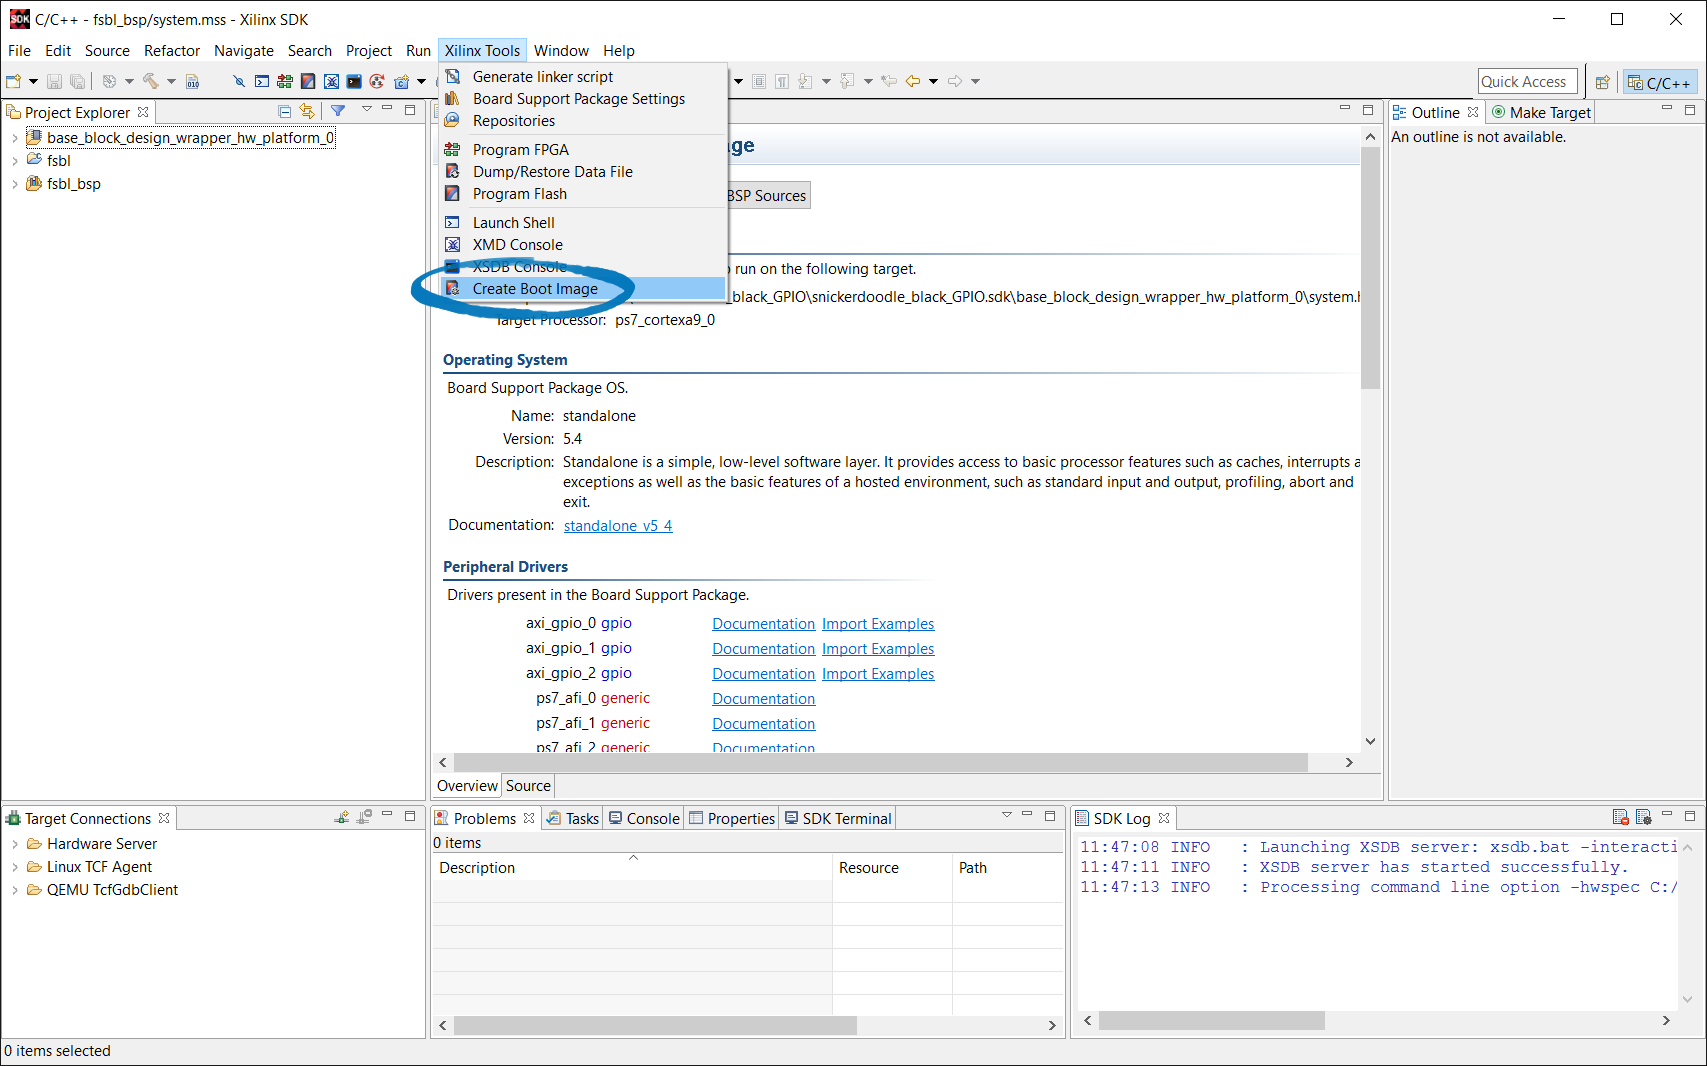
\includegraphics{images/sdk/create_boot_image_menu.png}
	\caption{Create Boot Image SDK Menu Selection}
	\label{fig:createbootimagemenu}
\end{figure}


The SDK provides a graphical way to select the components/partitions for the boot image and generate a reusable boot image file (\texttt{.bif}). The graphical front-end provides the necessary interface for selecting existing boot partitions (typically pre-compiled and/or provided by Vivado project) and will generate the \texttt{.bif} file along with the boot image. \figref{fig:createbootimage} shows the graphical interface for creating Zynq boot images from the SDK. To access the interface and begin generating images, select \menupath{Xilinx Tools, Create Boot Image} from the menubar in the SDK as shown in \figref{fig:createbootimagemenu}. \\



\begin{figure}
	\centering
	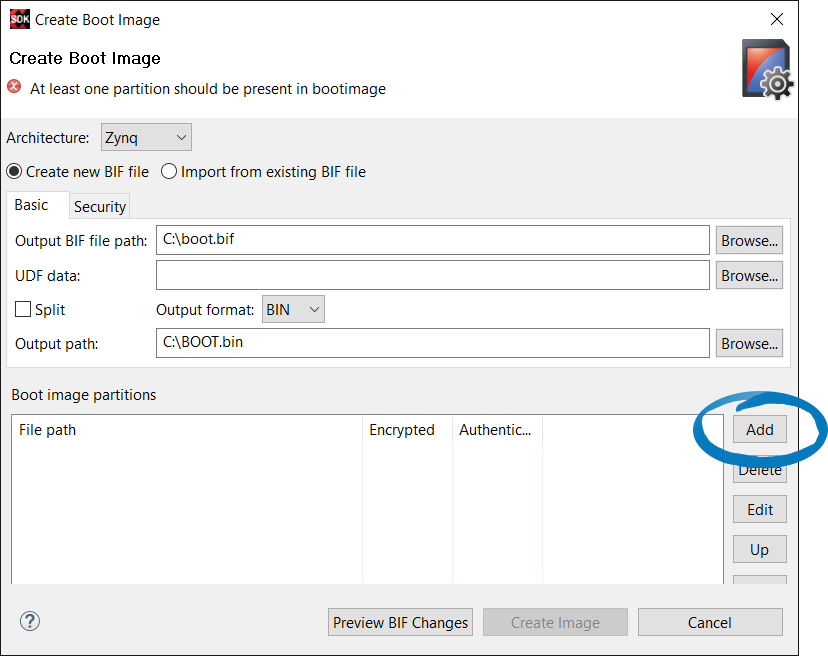
\includegraphics{images/sdk/create_boot_image.png}
	\caption{Create Boot Image Interface in Xilinx SDK}
	\label{fig:createbootimage}
\end{figure}


Prebuilt \texttt{.bif} files can be used by the SDK interface by selecting "Import from exisiting BIF file", shown at the top of the window in \figref{fig:createbootimage}. Boot partitions are listed in the "Boot image partitions" table within the interface. To add boot partitions from the interface, selecting "Add" will open an "Add partition" dialog (shown in \figref{fig:bootimagepartition}) which will allow you to select and specify the partition file.


\begin{marginfigure}
	\centering
	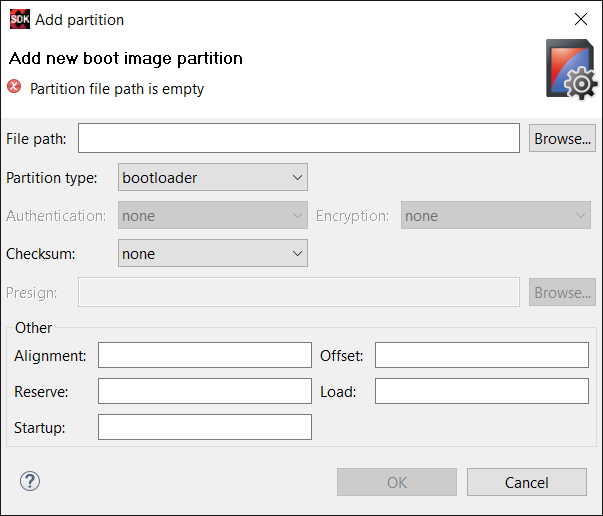
\includegraphics{images/sdk/boot_image_partition.png}
	\caption[Create New Boot Image Parition]{Create New Boot Image Parition}
	\label{fig:bootimagepartition}
\end{marginfigure}


%%%-------- Import and Specify Boot Images Sources ---------
\subsection{Import and Specify Boot Images Sources}

The most typical boot image for a Linux based system includes a FSBL, bitstream and U-Boot which will be used to load Linux. The image sources should be added one-by-one by clicking \textit{Add} from the \textit{Create Boot Image} interface as shown in \figref{fig:createbootimage}. FSBL should be specified as the bootloader by selecting \textit{bootloader} as the parition type as shown in \figref{fig:fsblbootimagepart}. \\


\begin{figure}
	\centering
	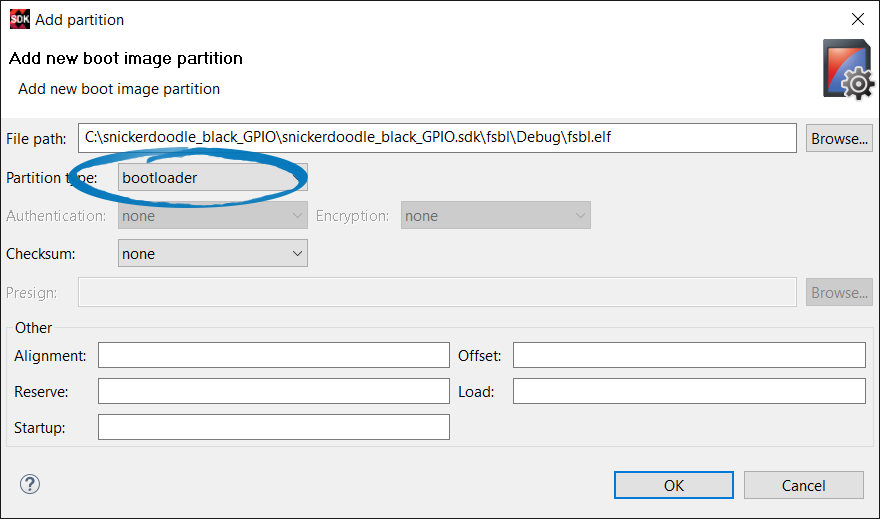
\includegraphics{images/sdk/fsbl_boot_partition.png}
	\caption{FSBL Bootloader Boot Image Partition}
	\label{fig:fsblbootimagepart}
\end{figure}


After adding the FSBL, add the bitstream and U-Boot images from the filesystem. Add the sources as a\textit{datafile} as shown in \figref{fig:ubootbootimagepart}. Prebuilt U-Boot executables can be downloaded from \href{https://github.com/krtkl}{GitHub} and copied to the workspace directory for import into boot image generation. Additional system components can be added in the same way and \textit{Offset} or \textit{Load} locations can be specified in the \textit{Add partition} dialog. \\


\begin{figure}
	\centering
	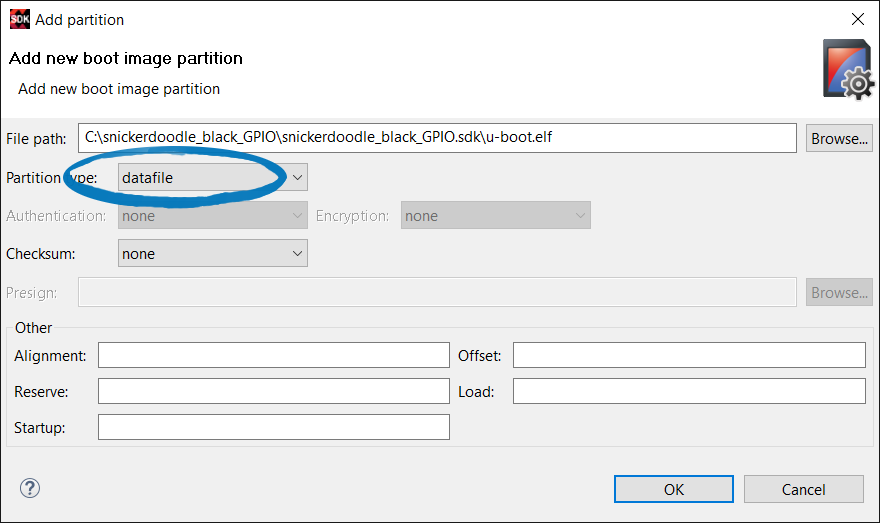
\includegraphics{images/sdk/u_boot_bootgen_partition.png}
	\caption[U-Boot Boot Image Partition Selection]{U-Boot Boot Image Partition Selection}
	\label{fig:ubootbootimagepart}
\end{figure}


After importing the boot image sources, the boot image interface should look similar to \figref{fig:bootimageparttable}. \\


\begin{figure}
	\centering
	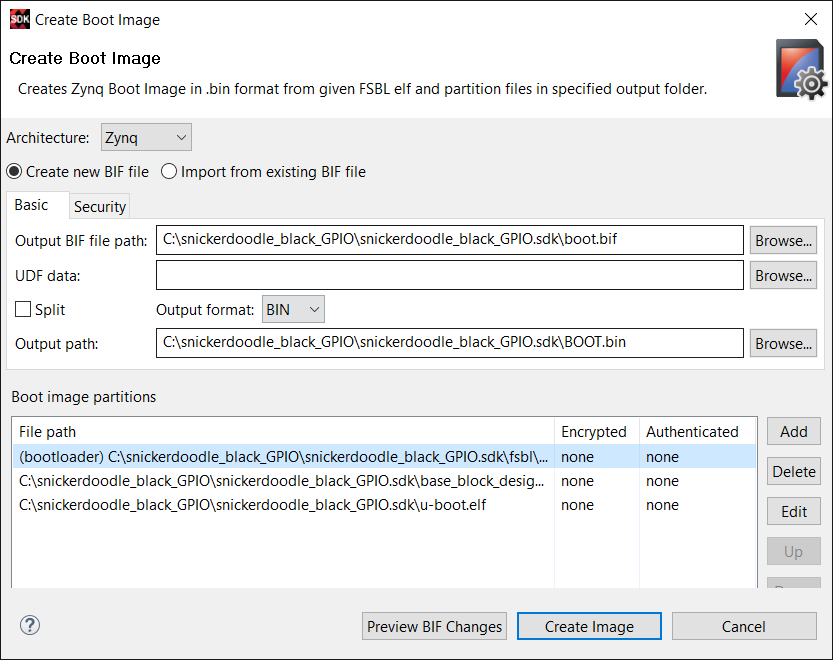
\includegraphics{images/sdk/create_boot_image_layout.png}
	\caption{Boot Image Partition Table}
	\label{fig:bootimageparttable}
\end{figure}


After selecting \menupath{Create Image}, the SDK console should output the status of the \texttt{bootgen} command and the generated boot image location. The generated boot image can then be loaded onto a microSD card and used as a boot source.


\begin{lstlisting}[%
	style=text,
	caption=SDK Create Boot Image Console Output
]
cmd /C bootgen -image boot.bif -arch zynq -o \
C:\snickerdoodle_black_GPIO\snickerdoodle_black_GPIO.sdk\BOOT.bin 
\end{lstlisting}


\subsection{Building Boot Images with \cmdstr{bootgen}}

\margincautionnote{When building boot images with \texttt{bootgen} the boot partition files and \texttt{.bif} file should be isolated in a working directory from which \texttt{bootgen} is executed.}

The GUI interface for building boot images from within the SDK is simply a wrapper for the command line executable that serves the same purpose. \texttt{bootgen} can be provided with a \texttt{.bif} file to specify the boot image partitions. Below is an example \texttt{.bif} file:

\begin{lstlisting}[
	style=text, 
	caption=Boot Information File
]
image : {
	[bootloader]fsbl.elf
	bitstream.bit
	u-boot.elf
}
\end{lstlisting}


After copying the boot partition file and the \texttt{.bif} file to a local working directory, the \texttt{bootgen} utility can be executed from that directory to output the boot image. Invoking the following command will create a boot image (\file{BOOT.bin}) using the boot image file \texttt{boot.bif}:


\begin{lstlisting}[%
	style=text,
	caption=Generate \texttt{BOOT.bin} with \texttt{bootgen}
]
$ bootgen -image boot.bif -o i BOOT.bin
\end{lstlisting}


\section{Linux}

\subsection{Device Tree}


Declaration of FPGA hardware peripherals in the device tree allows them to be configured and controlled by the Linux kernel using device drivers. This allows the control of the hardware to be abstracted to user-space using any of a number of interfaces including \texttt{sysfs}. The device tree node for a hardware peripheral specifies the device driver to use for hardware interfacing in the \texttt{compatible} parameter. The hardware register address space is declared in the \texttt{reg} parameter. 


\begin{lstlisting}[%
	style=text,
	caption=AXI GPIO IP Peripheral Device Tree Node,
	label=lst:gpiodtsnode]
gpio@41200000 {
	compatible = "xlnx,xps-gpio-1.00.a";
	gpio-controller;
	#gpio-cells = <0x2>;
	interrupt-parent = <0x3>;
	reg = <0x41200000 0x10000>;
	xlnx,is-dual = <0x0>;
	xlnx,all-inputs = <0x0>;
	xlnx,tri-default = <0xffffffff>;
	xlnx,gpio-width = <0x19>;
};
\end{lstlisting}

\begin{lstlisting}[%
	style=text,
	caption=AXI Timer (PWM) IP Peripheral Device Tree Node,
	label=lst:timerdtsnode]
timer@42800000 {
	clock-frequency = <50000000>;
	#pwm-cells = <0x2>;
	clocks = <0x1 15>;
	compatible = "xlnx,pwm-1.00";
	reg = <0x42800000 0x10000>;
};
\end{lstlisting}


The device driver will determine how the hardware peripheral is abstracted to user-space (if at all). In the case of the GPIO and AXI timer peripherals, the user-space abstraction is done through \texttt{sysfs}.


\subsection{Hardware Control and Observation in User Space}

Many hardware blocks can be controlled using built-in Linux drivers that abstract control of the hardware to file I/O. This allows interfacing with the hardware using a familiar Linux interface. The following code snippet shows an example routine for setting the value of a GPIO output pin by opening, writing to, and closing the \texttt{value} file of that pin in the GPIO subsystem of \texttt{sysfs}. 

\begin{fullwidth}
\begin{lstlisting}[language=C]
/**
  * @brief	Set GPIO Value
  *
  * @param  pin:	Pin ID to write value
  * @param  val:	Value to write to the output pin
  *			This parameter can have the following values:
  *			@arg GPIO_HIGH: Set the gpio output high
  *			@arg GPIO_LOW: Set the gpio output low
  * @retval 0 on success, error status otherwise
  */
int gpio_write(int pin, int val)
{
	int len, fid, status;
	char pin_path[BUFFER_LENGTH];
	char pin_val[2];

	len = snprintf(pin_path, BUFFER_LENGTH, "/sys/class/gpio/gpio%d/value", pin);

	fid = open(pin_path, O_WRONLY);

	if (fid < 0) {
		fprintf(stderr, "Failed to open GPIO %d value for writing\n", pin);
		return -1;
	}

	len = snprintf(pin_val, 2, "%d", val ? 1 : 0);

	status = write(fid, pin_val, len);

	if (status < 0) {
		fprintf(stderr, "Failed to set value for GPIO %d\n", pin);
		return -2;
	}

	close(fid);

	return 0;
}
\end{lstlisting}
\end{fullwidth}






